%%%%%%%%%%%%%%%%%%%%%%%%%%%%%%%%%%%%%%%%%%%%%%%%%%%%%%%%%%%%%%%%%%%%%%%%%%%%%%%%
%
%   Semester project, fall term 2014
%   Author: Jakob Ehrl, born 01/24/91
%   Study program: Computer science, MA 1
%   
%   Professor Dr. Francesco Mondada
%   Assistant: Dr. Stefan Witwicki
%
%%%%%%%%%%%%%%%%%%%%%%%%%%%%%%%%%%%%%%%%%%%%%%%%%%%%%%%%%%%%%%%%%%%%%%%%%%%%%%%%%

\chapter{Introduction}

\section{Description of the challenge}
This competition involves 5 teams of 3 students coming from different sections and aims to challenge the students in building  an autonomous mobile robot for PET bottles collection and transport in a reserved area.
In the figure below (Figure \ref{fig:Arena}) is represented the 8mx8m arena where the robot will have to work.
The arena is divided in 4 differents zones and, according to the difficulty to access or to perform in the zone, and the weight in terms of points accorded for each bottle collected is different.

\begin{figure}[H]
  \centering
  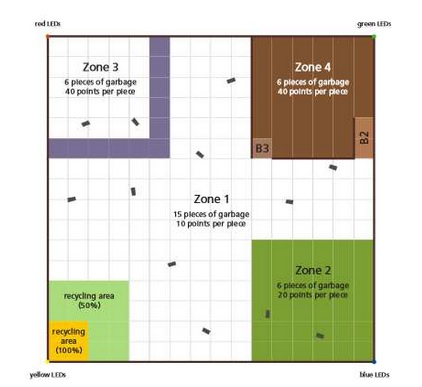
\includegraphics[width=0.6\textwidth]{Arena.jpg}
  \caption{Arena configuration.}
\label{fig:Arena}
\end{figure}

After being picked up the PET bottles need to be transported to a 1mx1m recycling area (left-down corner in Figure \ref{fig:Arena}) in order to be awarded with the 100\% of the points given by the bottles.
If they were to be released within the second limit of the recycling area they would be worth 50\% of the points. Finally if they were to be kept within the robot the amounts in points would be 25\% of the actual value of the collected bottle. 

%\chapter{Research}

%\section{Ideas}
%some drawings and stuff from the main ideas in the %beginning

\section{Selection process}

%(The tables where we chose the features of the robot, and the cahier des charges that we should respect)

Firstly, as a group, we evaluated all the possible strategies that could lead to the achievement of the goal.
In the following, can be found in a schematic way the charts describing the morphology of all the solutions that have been evaluated as well as the choices that brought us to the final design of our robot that will be treated in the following section.

This first chart (Figure \ref{fig:MechanicalChoices}) analyzes the possible solutions that we evaluated for the robot's locomotion. In particular, the wheeled solutions, refer to the use of the Wild thumper chassis that can be modified exploiting either 4 or 6 wheels. The Wild thumper chassis is easy to modify, add components to, since it has holes in it, and is a rather modular chassis, that can be modified, and decomposed into smaller parts. This chassis was the one present in the catalogue, therefore the easiest to obtain. Furthermore this kind of structure had been used also in the previous editions of the competition and this was a good basis in terms of experience to begin with. A custom chassis was also possible to obtain, since workshops were available to manufacture parts for the competition, however, the workload was already very high, and the workshops were already very busy and could only manufacture a very limited number of parts.
Others solutions like rubber tracks and swedish wheels have also been evaluated. However, as depicted in the related chart, the advantages in using the Wild Thumper chassis with 4 wheels resulted more appealing to us, in particular its polyvalence, making us pick up this solution for the robot’s locomotion.

\begin{figure}[H]
 \centering
 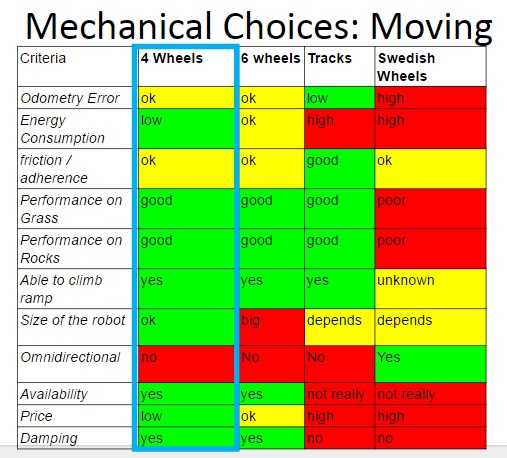
\includegraphics[width=0.7\textwidth]{MechanicalChoises.jpg}
 \caption{Morphological chart of the mechanical criteria.}
\label{fig:MechanicalChoices}
\end{figure}

The objective of the competition was the collection of bottles, so right after choosing the locomotion method we started evaluating the possible solutions to accomplish this goal.
The first evaluation we made has been about the principle behind the system.
Indeed there are two possible approaches to the achievement of this task:

\begin{itemize}
\item Selective Approach
\item Greedy Approach
\end{itemize}

In a selective approach, each bottle has to be detected and, furthermore, its position and orientation need to be computed in order to approach the PET bottle in the desired way and grasping it by mean of a robotic arm or another precise pick up system (see the solution of group 3). 
However, this kind of solution, even if fascinating, appeared to us as a constraint and would have inevitably led to a too high workload. 
As the duration of the competition was only 10 minutes, we assumed that a selective approach was too slow to pick up many bottles in such a short time. Thus we pointed toward a more greedy approach.
In a greedy approach, bottles don’t need to be perfectly identified and they could be picked up also by only being in the path of the robot.
With this idea in mind we started evaluating the mechanic systems that could provide such a favorable behavior.
The evaluated solutions are shown in the chart in Figure \ref{fig:PickUpApproach}.
In our case we have chosen to couple a rigid elevator, which aims to pick up the bottle from the terrain putting it in a storage area upon the robot, with a rotating sponge, as the ones used for painting walls, represented in figure \ref{fig:PickUpChoices} that aims to push the bottle within the elevator and avoid to make it exit once entered. 

\begin{figure}[H]
 \centering
 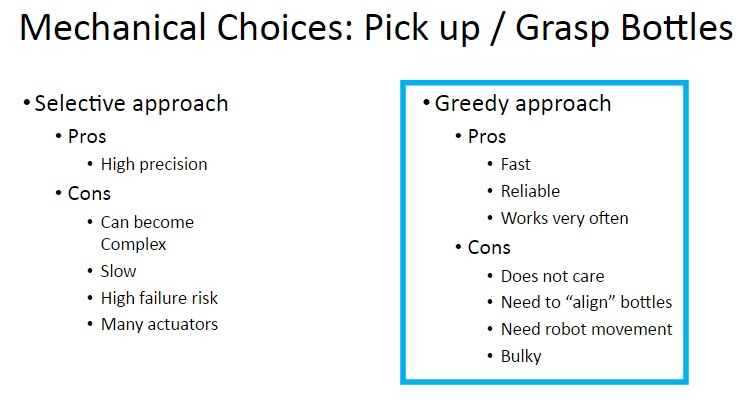
\includegraphics[width=0.9\textwidth]{PickUpApproach.jpg}
 \caption{Possible approaches for picking up a bottle.}
\label{fig:PickUpApproach}
\end{figure}

\begin{figure}[H]
 \centering
 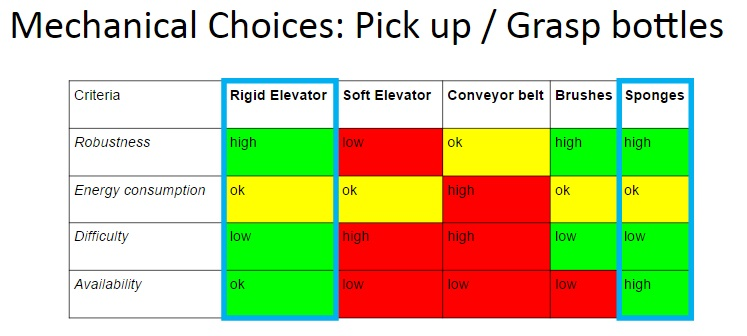
\includegraphics[width=0.9\textwidth]{PickUpChoises.jpg}
 \caption{Chart of the picking up criteria.}
\label{fig:PickUpChoices}
\end{figure}

The bottles, once collected, are placed in a storage area disposed on the robot chassis. To chose the size of the robot, we used the chart \ref{fig:TransportBottles}.

\begin{figure}[H]
 \centering
 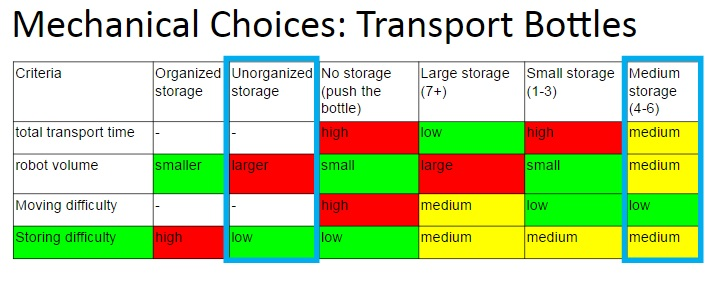
\includegraphics[width=0.8\textwidth]{TransportBottles.jpg}
 \caption{Chart of the possible solutions to transport the bottles.}
\label{fig:TransportBottles}
\end{figure}

Finally, in figure \ref{fig:ObjectDetection} is shown the chart that made us choose the sensors that allows the robot to perceive the environment and detect the bottles.                                                
\begin{figure}[H]
 \centering
 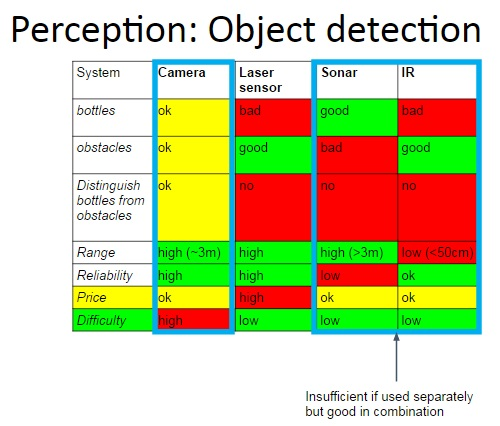
\includegraphics[width=0.7\textwidth]{ObjectDetection.jpg}
 \caption{Morphological chart for the sensors choice.}
\label{fig:ObjectDetection}
\end{figure}

\section{Division of labor}
Initially, in order to speed up the robot’s process of realization we distributed the principal tasks among the members of the team.
Three main tasks were given, one for each member of the team, in order to work in parallel, to fulfill the goal faster. These tasks were:

\begin{itemize}
\item Mechanical Part : \textit{developpment of the mechanical aspect of the robot, creation of a solidworks model, and drawings for the mechanical workshop.}
\item Electronic Part : \textit{Choice of the power, electronic components, soldering, testing and connections.}
\item Software Part : \textit{developpmemt of the algorithm, the communication protocols, image processing and scripts.}
\end{itemize}

Challenges of such an project was to respect these charts as much as possible and to stick to the plan. As it was suggested by the assistants, the evaluated time is always too short for a specific task, and the  difficult task was to determine exactly how much time a certain task or accomplishement would take. \\

Deadlines on achievements for each single part were defined according to Gantt charts that helped us to keep an overall look on the advancement of the project.
In the Annex is represented the first Gantt chart conceived after the decision on the main characteristics of the robot and previous to the last milestone were all the details behind our idea of the robot were to be discussed with the supervisors.\\

Another Gantt chart has been realized after the 3th milestone in order to organize the final work and it is showed in the Annex.\\

The division of the development of the robot in mechanical, electronic and software aspect was necessary to speed up the realization of the robot, although the lasts weeks have been dedicated to the merging of these differents parts allowing the team to work on the mechatronic of the robot and finally obtaining it with all the characteristics that had emerged during the initial brainstorming and developped during the advancement of the single parts.